\documentclass{beamer}

\mode<presentation> {
\usetheme{Madrid}
}

\usepackage{graphicx}
\usepackage{svg}
\usepackage{booktabs}
\usepackage{amsmath}
\usepackage[french]{babel}
\usepackage{url,color}
\usepackage{subfigure}
\usepackage{amsthm,amsfonts,amssymb,amscd,amsxtra, multicol}
\usepackage{comment}

\graphicspath{ {./images/} }

% \setbeamertemplate{caption}[numbered]
% \newcommand{\tabitem}{~~\llap{\textbullet}~~}

\title{Conception d'un SaaS pour les cours en ligne en milieu universitaire}
\author[Hans TOGNON]{Hans B. K. \textbf{TOGNON} \\ Supervisé par Ing. Miranda \textbf{GNONLONFOUN}}
\institute[IFRI]{
\textbf{I}nstitut de \textbf{F}ormation et de \textbf{R}echerche en  \textbf{I}nformatique \\
\medskip
% \textbf{\color{magenta}\href{mailto:contact@ifri.uac.bj}{contact@ifri.uac.bj}}
}

\begin{document}
% %%%%%%%%%%%%%%%%%%%%%%%%%%%%%%%%%%
% Title Page
% %%%%%%%%%%%%%%%%%%%%%%%%%%%%%%%%%%
\begin{frame}
  \thispagestyle{empty}
  \begin{multicols}{2}
    \begin{figure}
        \flushleft
        
\includegraphics[width=0.11\textwidth]{logoifri}
    \end{figure}
    \begin{figure}
        \flushright
        
\includegraphics[width=0.1\textwidth]{logouac}
    \end{figure}
    \end{multicols}
    \vspace{-1cm}
  \titlepage
  \end{frame}

% %%%%%%%%%%%%%%%%%%%%%%%%%%%%%%%%%%
% ToC
% %%%%%%%%%%%%%%%%%%%%%%%%%%%%%%%%%%
\begin{frame}
  \frametitle{PLAN}
  \begin{itemize}
    \item Introduction
    \item Revue de Littérature
    \item Matériels et méthodes
    \item Résultats \& Discussion
    \item Conclusion \& Perspectives
  \end{itemize}
\end{frame}

% %%%%%%%%%%%%%%%%%%%%%%%%%%%%%%%%%%
% Introduction
% %%%%%%%%%%%%%%%%%%%%%%%%%%%%%%%%%%


% %%%%%%%%%%%%%%%%%%%%%%%%%%%%%%%%%%
% Revue de Littérature
% %%%%%%%%%%%%%%%%%%%%%%%%%%%%%%%%%%

% %%%%%%%%%%%%%%%%%%%%%%%%%%%%%%%%%%
% Matériels et méthodes
% %%%%%%%%%%%%%%%%%%%%%%%%%%%%%%%%%%
\begin{frame}{Matériels et Méthodes : \small{UML} - \footnotesize{Diagramme de cas d'utilisation}}
  \begin{figure}[H]
    \centering
    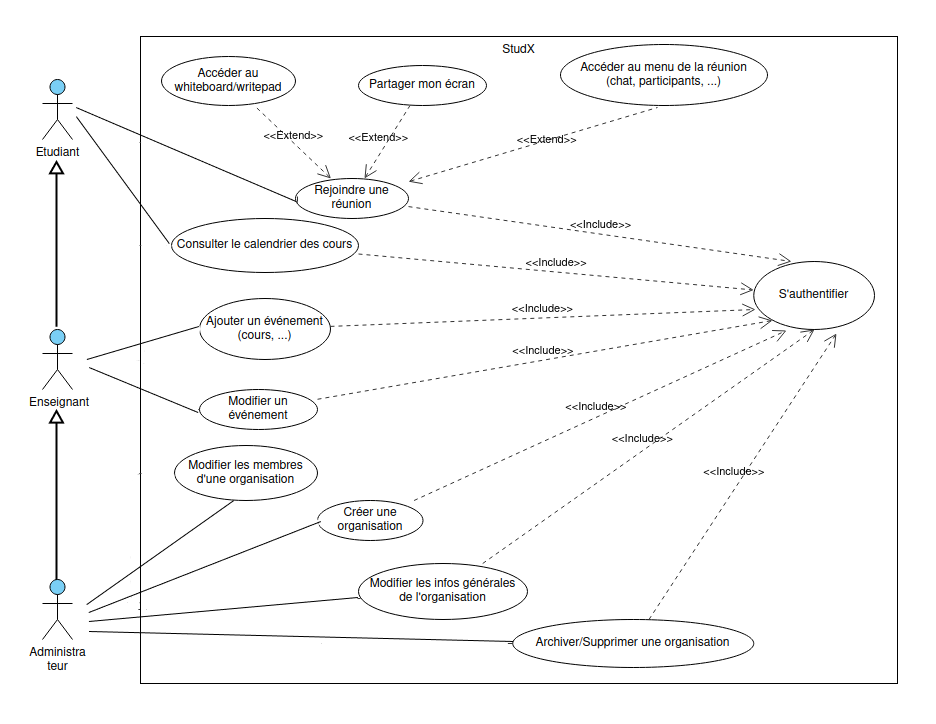
\includegraphics[width=\textwidth]{../../images/use-cases-diag.png}
    \caption{Cas d'utilisation}
\end{figure}

\end{frame}

\begin{frame}{Matériels et Méthodes : \small{UML} - \footnotesize{Diagramme de classe}}
  \begin{figure}[H]
    \centering
    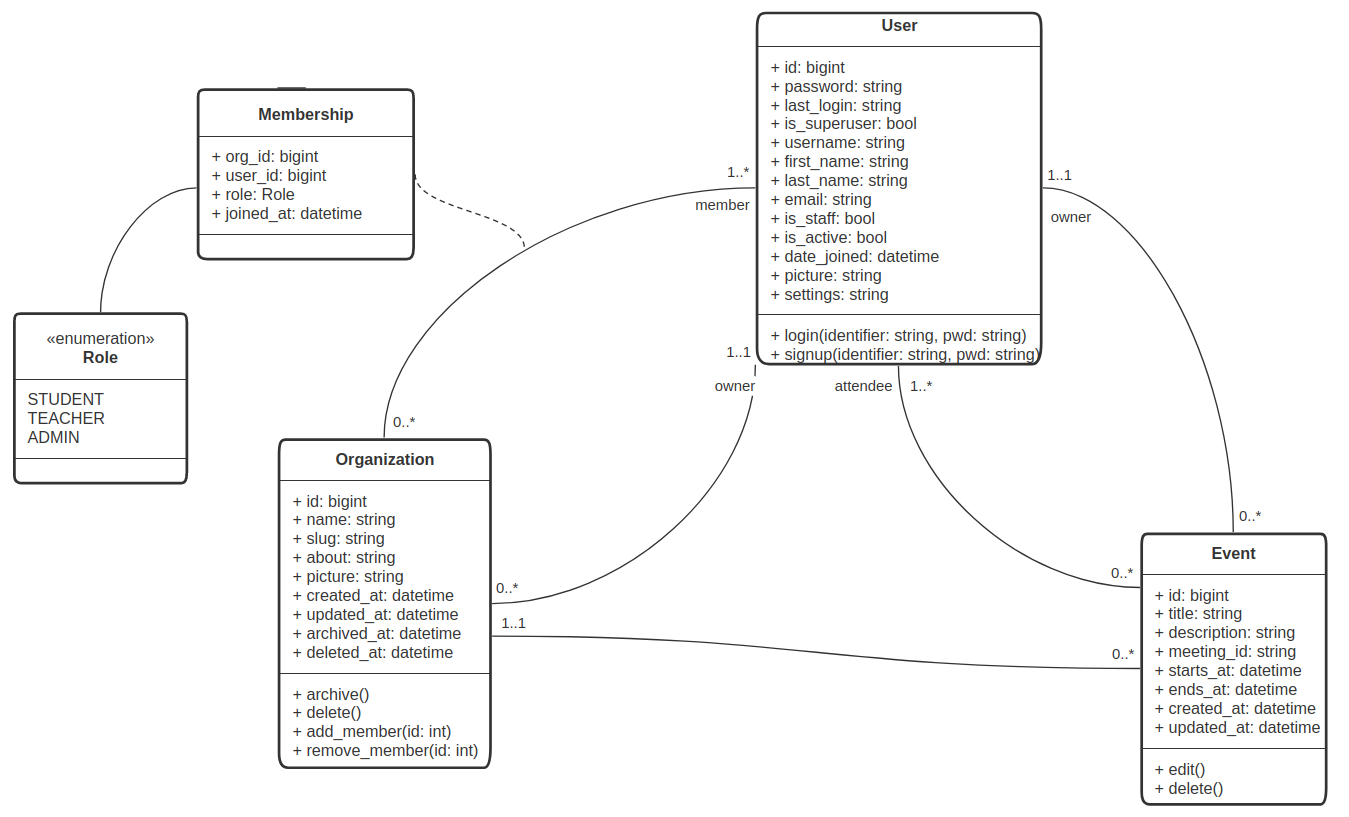
\includegraphics[width=\textwidth]{../../images/class-diag.png}
    % \caption{Diagramme de classe}
\end{figure}
\end{frame}

\begin{frame}{Matériels et Méthodes : \small{UML} - \footnotesize{Diagramme de séquence}}
  \begin{figure}[H]
    \centering
    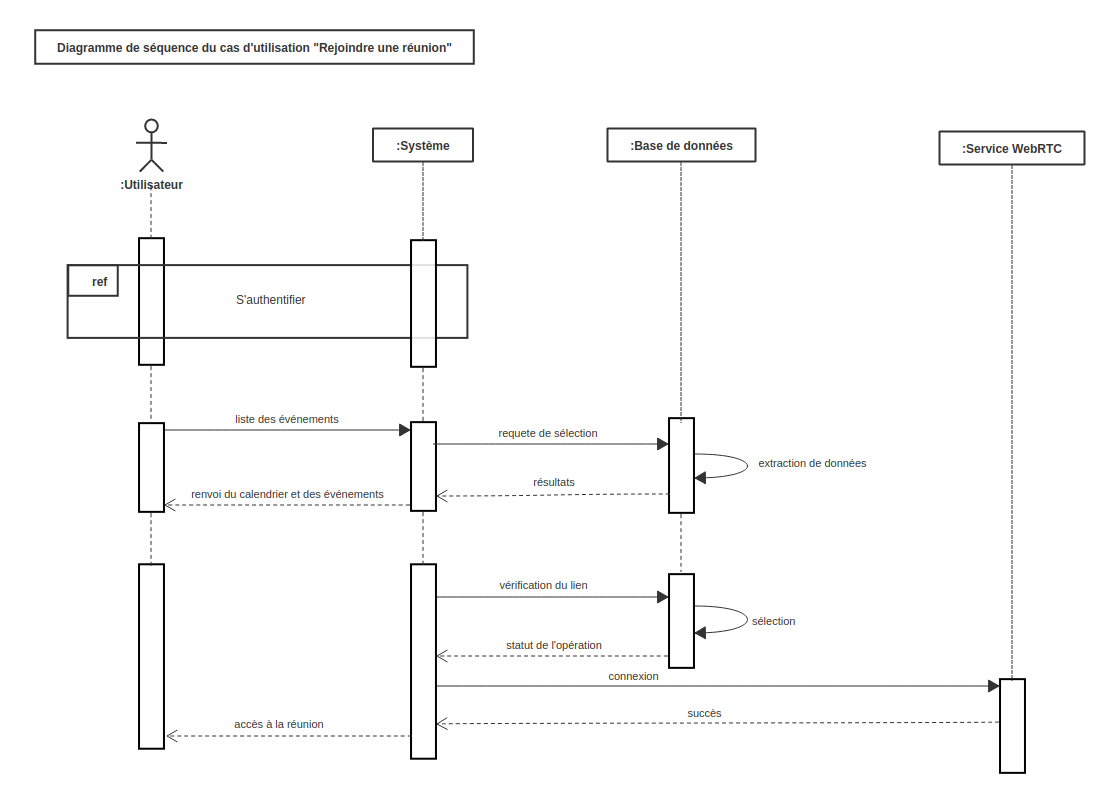
\includegraphics[width=0.9\textwidth]{../../images/join-meet-sequence-diag.png}
    % \caption{Diagramme de séquence (fonctionnalité principale)}
\end{figure}
\end{frame}

\begin{frame}{Matériels et Méthodes : \small{UML} - \footnotesize{Architecture Logicielle}}
  \begin{figure}[H]
    \centering
    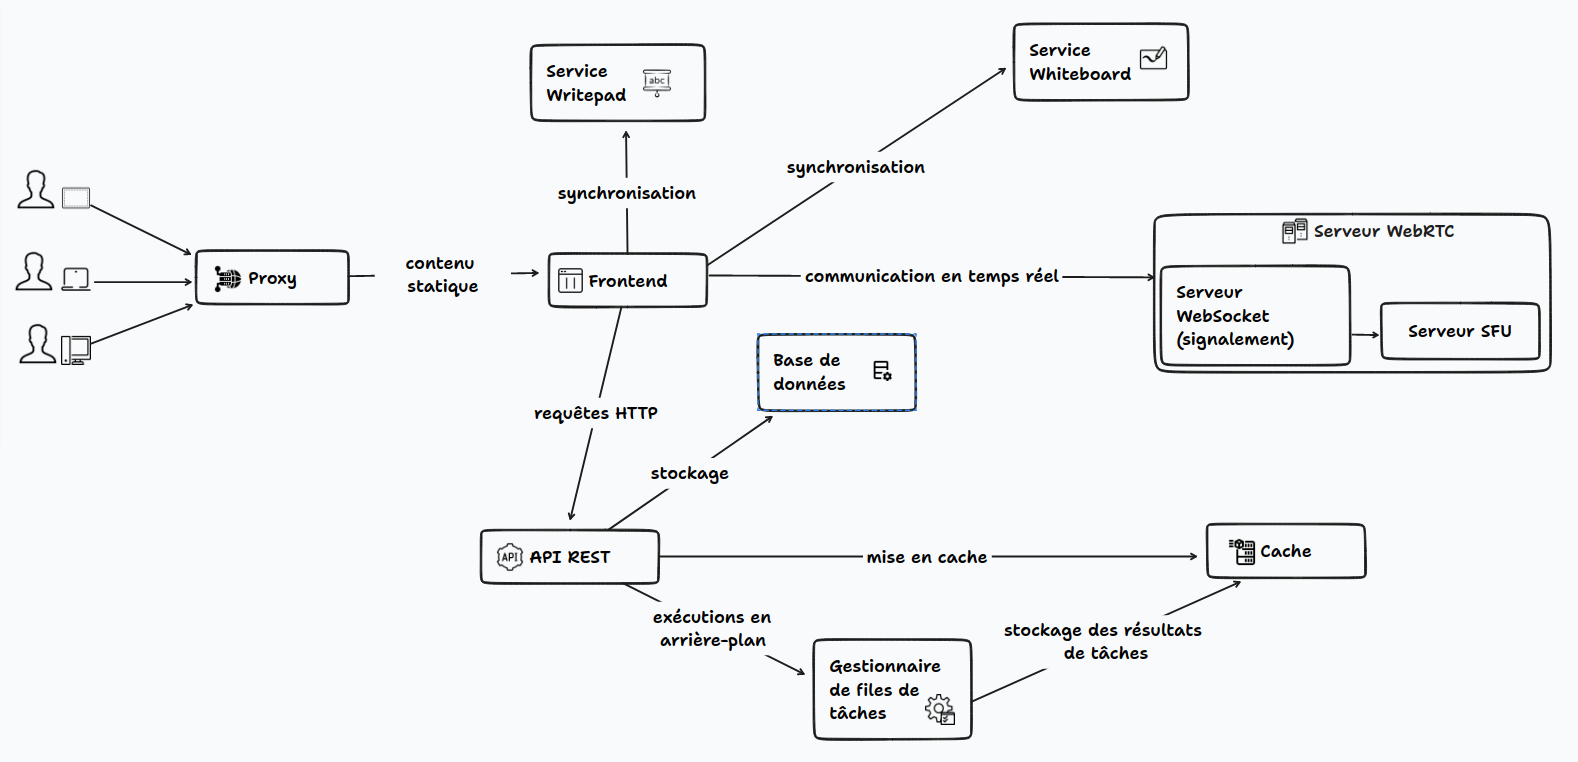
\includegraphics[width=\textwidth]{../../images/studx-system-design}
\end{figure}
\end{frame}

\begin{frame}{Matériels et Méthodes : \small{Technologies}}
  \begin{figure}[H]
    \centering
    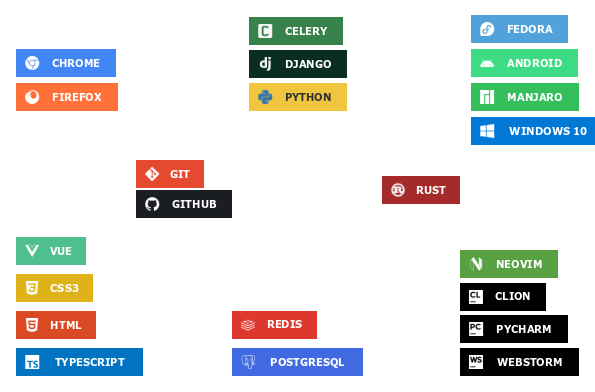
\includegraphics[width=0.9\textwidth]{tools}
    % \caption{Outils technologiques}
\end{figure}
\end{frame}


% %%%%%%%%%%%%%%%%%%%%%%%%%%%%%%%%%%
% Résultats et Discussion
% %%%%%%%%%%%%%%%%%%%%%%%%%%%%%%%%%%
\begin{frame}{Résultats : \small{Quelques Interfaces} }
  \begin{figure}[ht]
    \begin{minipage}[b]{0.45\linewidth}
        \centering
        \frame{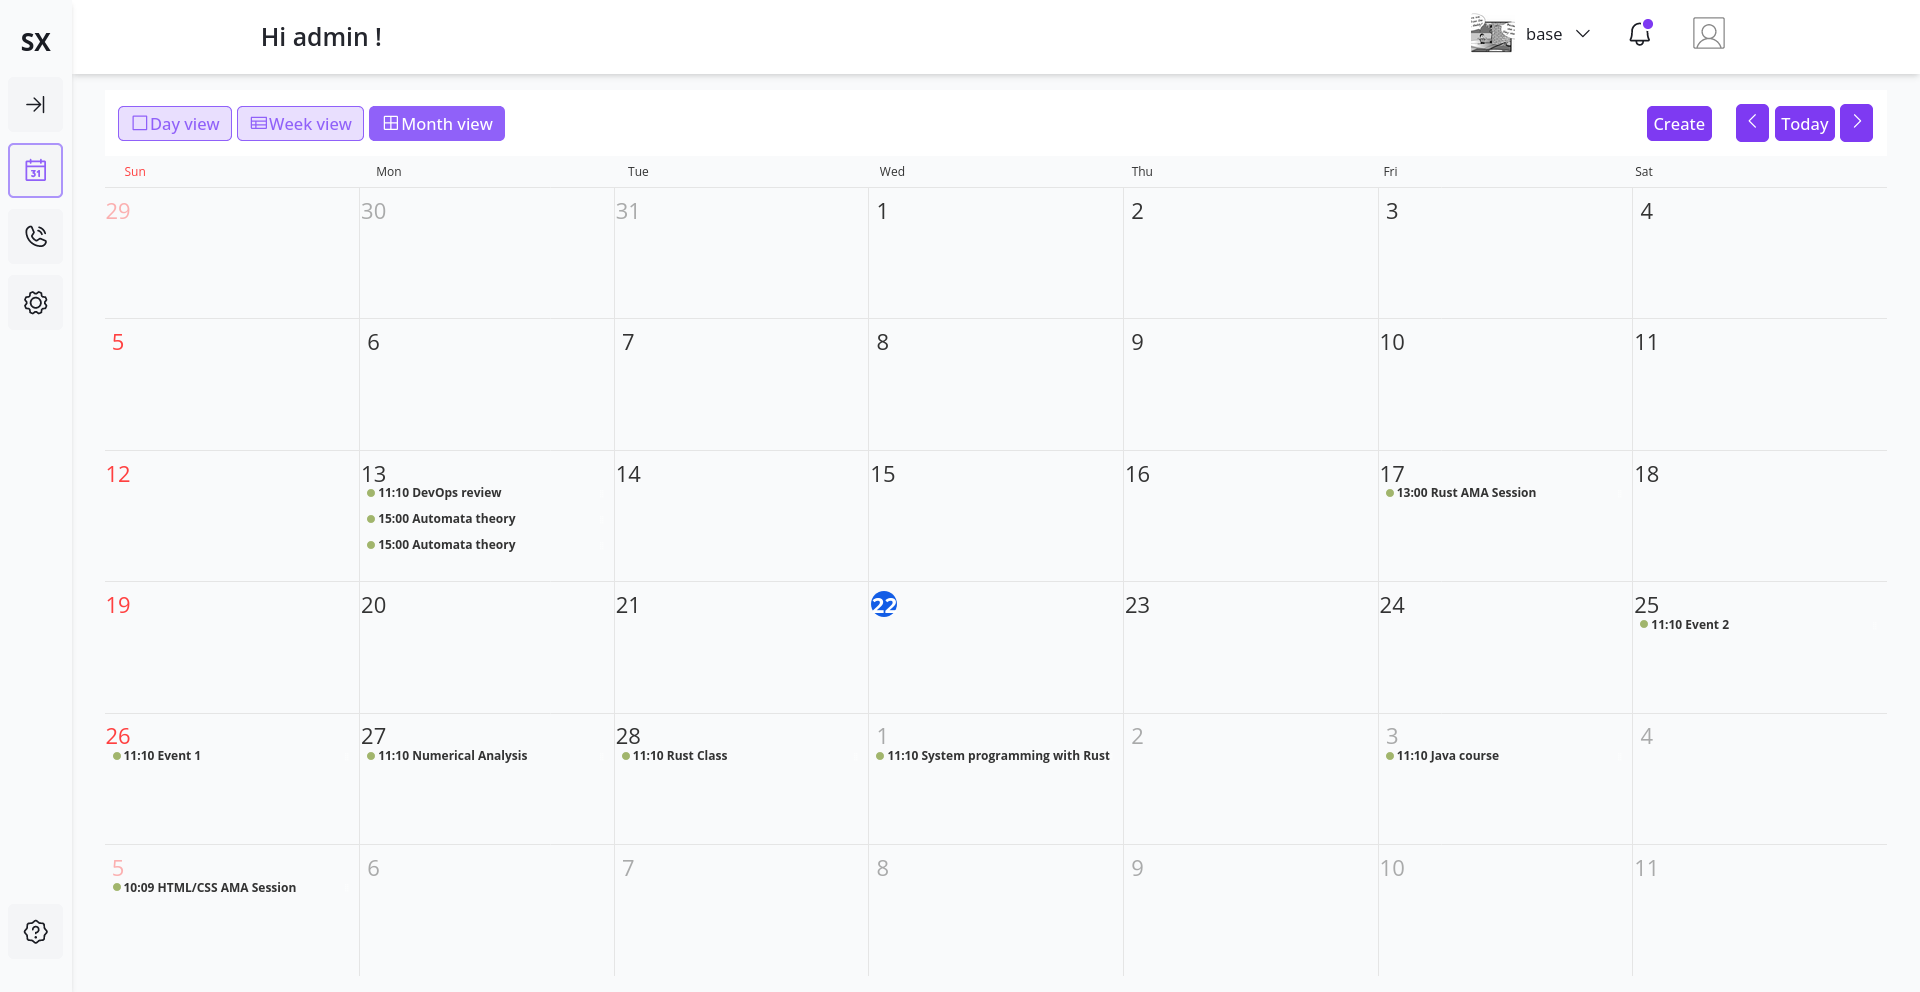
\includegraphics[width=\textwidth]{../images/prototype/calendar-view}}
        \label{fig:a}
    \end{minipage}
    \hspace{0.5cm}
    \begin{minipage}[b]{0.45\linewidth}
        \centering
        \frame{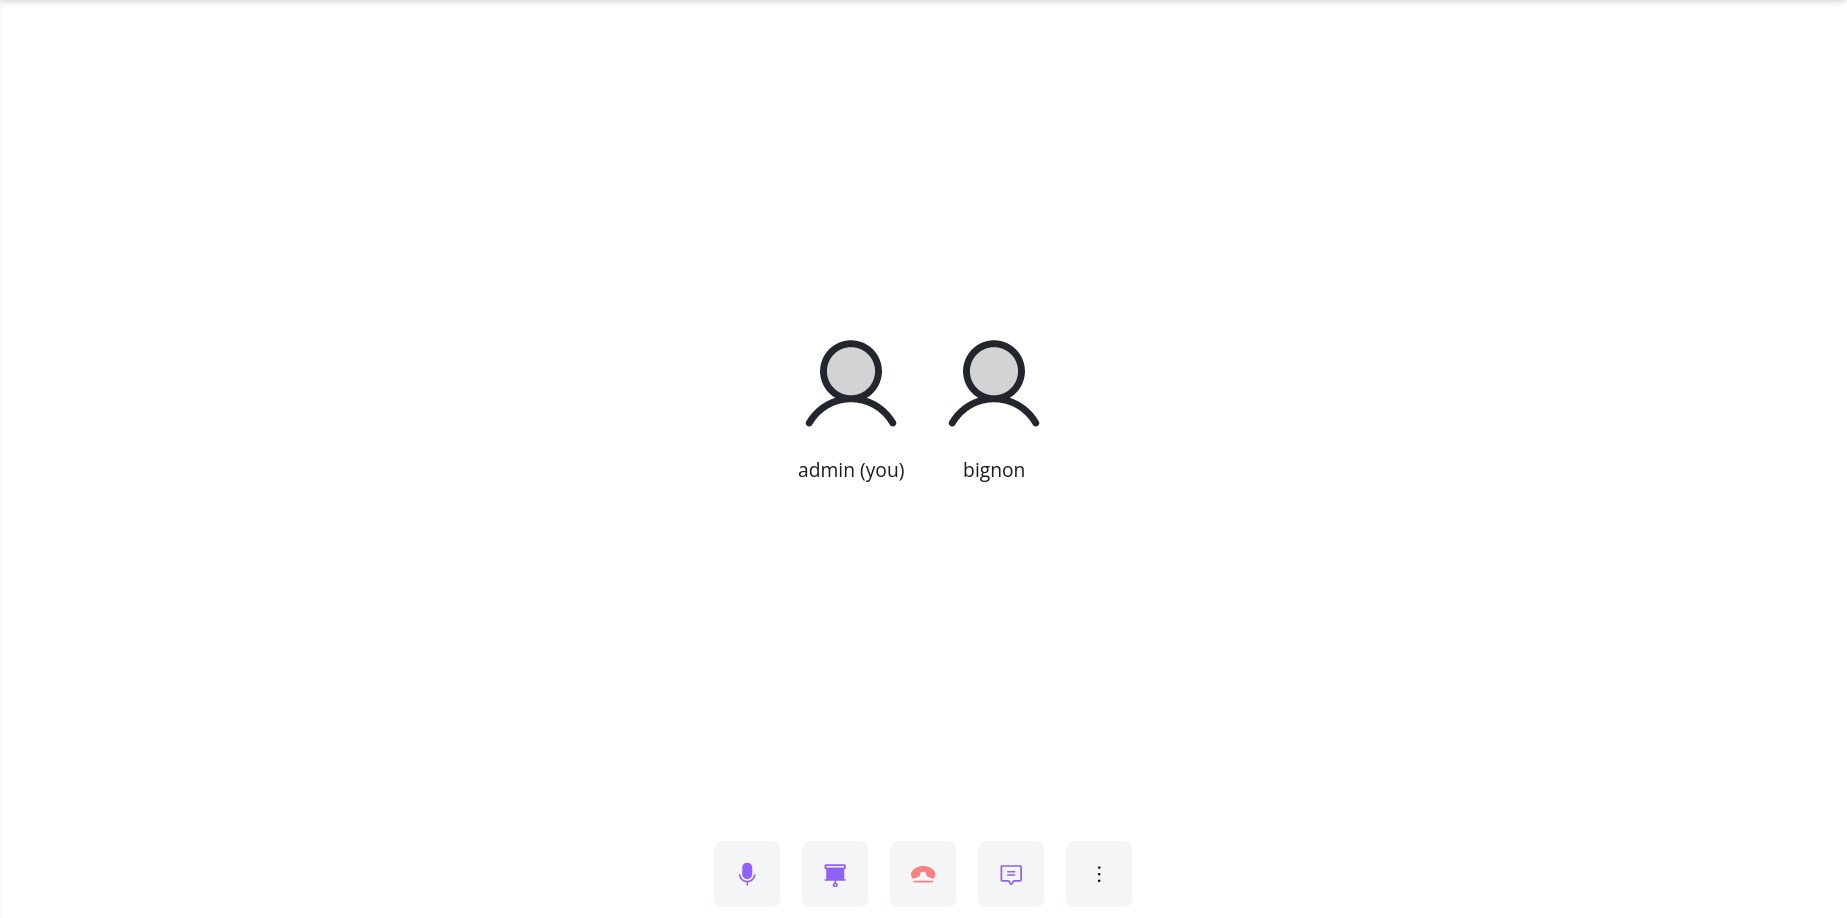
\includegraphics[width=\textwidth]{../images/prototype/user-with-participants-in-room}}
        \label{fig:b}
    \end{minipage}
\end{figure}
\end{frame}

\begin{frame}{Résultats \& Discussion}
  \begin{center}
    \Huge{Démonstration !}
  \end{center}
\end{frame}

\begin{frame}{Résultats \& Discussion}
\end{frame}

% %%%%%%%%%%%%%%%%%%%%%%%%%%%%%%%%%%
% Conclusion et Perspectives
% %%%%%%%%%%%%%%%%%%%%%%%%%%%%%%%%%%
\begin{frame}{Conclusion \& Perspectives}
\end{frame}

\begin{frame}{Conclusion \& Perspectives}
\end{frame}

% Thanks
\begin{frame}
  \begin{center}
  \Huge{Merci !}
  \end{center}

\end{frame}

\end{document}
